\documentclass[12pt, a4paper]{report}
\usepackage{graphicx}
\usepackage{amsmath}
\usepackage{float}
\usepackage{geometry}
\usepackage{fancyhdr}
\usepackage[portuguese]{babel}
\usepackage[utf8]{inputenc}

% Configurações de Margens
\geometry{left=3cm,right=2cm,top=3cm,bottom=2cm}

% Cabeçalhos e rodapés
\pagestyle{fancy}
\fancyhf{}
\fancyhead[L]{Universidade Federal do Tocantins}
\fancyhead[R]{Uma Rápida Análise de Algoritmos de Ordenação}
\fancyfoot[C]{\thepage}

% Início do Documento
\begin{document}

% Capa
\begin{titlepage}
    \centering
    
\includegraphics[width=0.3\textwidth]{uft_logo.png}\\[1cm]
    \vspace{1cm}
    \textbf{\Large UNIVERSIDADE FEDERAL DO TOCANTINS}\\[0.5cm]
    \textbf{\large CURSO DE GRADUAÇÃO EM CIÊNCIA DA COMPUTAÇÃO}\\[2cm]
    
    \textbf{\large Danilo Maciel\\Micael Ribeiro}\\[2cm]
    
    \textbf{\LARGE Uma Rápida Análise de Algoritmos de Ordenação}\\[7cm]
    
    Palmas, TO\\
    2025
    
\end{titlepage}

% Resumo
\chapter*{Resumo}
Nosso objetivo aqui é comparar o desempenho dos seis principais algoritmos de ordenação — Bubble Sort, Selection Sort, Insertion Sort, Merge Sort, Quick Sort e Heap Sort — por meio de testes com listas de diferentes tamanhos (1.000 a 100.000 elementos) e distribuições (ordenadas, inversas e aleatórias). Foram analisados tempo de execução, número de comparações e trocas. Os resultados indicam melhor desempenho do Heap Sort e Merge Sort em listas grandes, enquanto os algoritmos simples tiveram baixo desempenho

\vspace{0.5cm}

\textbf{Palavras-chave:} Bubble Sort. Selection Sort. Insertion Sort. Merge Sort. Quick Sort.  Heap Sort. Tempo de Execução. Ordenação. 

% Abstract
\chapter*{Abstract}
Our goal here is to compare the performance of the six main sorting algorithms — Bubble Sort, Selection Sort, Insertion Sort, Merge Sort, Quick Sort, and Heap Sort — through tests with lists of varying sizes (from 1,000 to 100,000 elements) and distributions (sorted, reverse, and random). Execution time, number of comparisons, and swaps were analyzed. The results indicate better performance by Heap Sort and Merge Sort on large lists, while the simpler algorithms showed lower performance.

\vspace{0.5cm}

\textbf{Keywords:} Sorting Algorithms. Empirical Analysis. Execution Time.

% Introdução
\chapter{Introdução}
A ordenação de dados é essencial para o funcionamento de sistemas no mundo moderno, impactando diretamente o desempenho de aplicações que lidam com grandes volumes de dados. A escolha do algoritmo adequado depende tanto do tamanho quanto da disposição dos dados, como listas ordenadas, invertidas ou aleatórias. Esta pesquisa analisa empiricamente seis algoritmos — Bubble Sort, Selection Sort, Insertion Sort, Merge Sort, Quick Sort e Heap Sort — considerando entradas de 1.000 a 100.000 elementos em diferentes distribuições. Os testes avaliam tempo de execução, número de comparações e trocas, permitindo comparar o desempenho e a eficiência de cada método em diferentes cenários.

% Revisão Teórica
\chapter{Visão geral}
\section{Bubble Sort}
Embora seja um dos algoritmos de ordenação mais fáceis de entender, o Bubble Sort apresenta um trade-off entre simplicidade e eficiência. Sua abordagem de comparar e permutar vizinhos resulta em uma complexidade de tempo de O(n²) para o caso médio e pior, limitando sua aplicabilidade em conjuntos de dados extensos. No entanto, sua performance melhora significativamente para O(n) em listas já ordenadas.

\section{Selection Sort}
Diferentemente do Bubble Sort, cuja performance varia conforme a entrada, o Selection Sort apresenta uma complexidade de tempo uniforme de O(n²). Seu funcionamento envolve a seleção contínua do menor ou maior item não ordenado e sua subsequente movimentação para a seção ordenada da lista.

\section{Insertion Sort}
O Insertion Sort ordena como organizar cartas, inserindo cada elemento na posição correta da sublista ordenada à esquerda. Simples de implementar e eficiente para listas pequenas ou quase ordenadas (O(n) no melhor caso). É um algoritmo in-place e estável. Contudo, para listas grandes e aleatórias, sua complexidade é O(n²), tornando-o menos eficiente que outros algoritmos avançados. Ideal para poucos dados ou inserção contínua.O Insertion Sort ordena como organizar cartas, inserindo cada elemento na posição correta da sublista ordenada à esquerda. Simples de implementar e eficiente para listas pequenas ou quase ordenadas (O(n) no melhor caso). É um algoritmo in-place e estável. Contudo, para listas grandes e aleatórias, sua complexidade é O(n²), tornando-o menos eficiente que outros algoritmos avançados. Ideal para poucos dados ou inserção contínua.

\section{Merge Sort}
\begin{itemize}
  \item \textbf{Tipo:} Algoritmo de ordenação por divisão e conquista.
  \item \textbf{Funcionamento:} Divide recursivamente o array em duas metades até que cada subarray tenha um único elemento.
  \item \textbf{Combinação:} As sublistas são então fundidas (merge) em ordem crescente.
  \item \textbf{Complexidade:} $O(n \log n)$ em todos os casos (melhor, médio e pior).
  \item \textbf{Estável:} Sim – mantém a ordem relativa dos elementos iguais.
  \item \textbf{Espaço extra:} Requer espaço adicional proporcional a $n$ para o array temporário.
\end{itemize}


\section{Quick Sort}
\begin{itemize}
  \item \textbf{Tipo:} Algoritmo de ordenação por divisão e conquista.
  \item \textbf{Funcionamento:} Escolhe um pivô, particiona os elementos menores à esquerda e maiores à direita.
  \item \textbf{Recursão:} Aplica o mesmo processo recursivamente às sublistas.
  \item \textbf{Complexidade:} Melhor e médio caso: $O(n \log n)$; pior caso: $O(n^2)$.
  \item \textbf{Estável:} Não – pode trocar a ordem de elementos iguais.
  \item \textbf{Espaço extra:} $O(\log n)$ no caso médio (devido à pilha de recursão).
\end{itemize}

\section{Heap Sort}
\begin{itemize}
  \item \textbf{Tipo:} Algoritmo de ordenação baseado em estrutura de heap binário.
  \item \textbf{Funcionamento:} Constrói um heap máximo, depois extrai repetidamente o maior elemento.
  \item \textbf{Etapas principais:} Construção do heap e ordenação por remoção da raiz.
  \item \textbf{Complexidade:} Sempre $O(n \log n)$, em todos os casos.
  \item \textbf{Estável:} Não – pode trocar a ordem de elementos iguais.
  \item \textbf{Espaço extra:} $O(1)$ – feito in-place, sem uso adicional de memória.
\end{itemize}


% Metodologia
\chapter{Metodologia}
\section{Hardware e software}
\begin{itemize}
    \item Notebook Dell Core i5 12500H
    \item 16 GB RAM DDR5
    \item Windows 11 Pro
    \item Ambiente de desenvolvimento: VS Code
    \item Linguagem: Python 3.12
\end{itemize}

\section{Implementação dos Algoritmos}
Os seis algoritimos de ordenação: Bubble Sort,
Selection Sort, Insertion Sort, Merge Sort, Quick Sort e Heap Sort foram implementados em linguagem python e de forma individual, para que o comportamento de cada um seja analisado de maneira independente.
\subsection*{Descrição dos Algoritmos:}

\begin{enumerate}
    \item \textbf{Bubble Sort:}
    \begin{itemize}
        \item A cada iteração, o algoritmo compara dois elementos adjacentes e os troca de lugar se estiverem fora de ordem. O processo é repetido até que a lista esteja completamente ordenada.
        \item \textbf{Complexidade:} O($n^2$) no pior caso e liner (n) no melhor caso
    \end{itemize}

    \item \textbf{Selection Sort:}
    \begin{itemize}
        \item O algoritmo encontra o menor elemento da lista e o move para a primeira posição. Em seguida, repete o processo para o restante da lista até que ela esteja ordenada.
        \item \textbf{Complexidade:} O($n^2$) em todos os casos 
    \end{itemize}

    \item \textbf{Insertion Sort:}
    \begin{itemize}
        \item O algoritmo percorre a lista, inserindo cada elemento em sua posição correta, movendo os elementos maiores para a direita conforme necessário.
        \item \textbf{Complexidade:} O($n^2$)no pior caso e linear (n) no melhor
    \end{itemize}

    \item \textbf{Merge Sort:}
    \begin{itemize}
        \item Merge Sort é um algoritmo de ordenação do tipo divide e conquista, que divide recursivamente a lista em sublistas até que cada uma contenha um único elemento, e então as combina em ordem. Ele é estável e eficiente para grandes volumes de dados. 
        \item \textbf{Complexidade:} O($n \log n$) sempre
    \end{itemize}

    \item \textbf{Quick Sort:}
    \begin{itemize}
        \item O algoritmo seleciona um pivô, particiona a lista em dois grupos (menores e maiores que o pivô), e ordena recursivamente cada parte.
        \item \textbf{Complexidade:} O($n \log n$) em média, e O($n^2$) no pior caso, dependendo da escolha do pivô.
    \end{itemize}

    \item \textbf{Heap Sort:}
    \begin{itemize}
        \item Heap Sort é um algoritmo de ordenação que transforma a lista em uma estrutura de heap (geralmente um max-heap) e então extrai o maior elemento repetidamente para ordenar os dados. É eficiente e não utiliza espaço adicional significativo. 
        \item \textbf{Complexidade:} O($n \log n$) sempre
    \end{itemize}
    
    
\end{enumerate}
No python usamos a classe SortMetrics() para salvar o número de comparações e trocas realizadas por cada um dos algoritmos 


\section{Procedimento para Medir Desempenho}
Os dados coletados durante a execução são:
\begin{itemize}
    \item \textbf{Tempo de execução:} Em Segundos.
    \item \textbf{Número de comparações:} Quantidade de Comparações na execução.
    \item \textbf{Número de trocas:} Quantidade de trocas durante a execução.
\end{itemize}

\subsection*{Medição}

Para avaliar o desempenho dos algoritmos de ordenação, implementamos um sistema automatizado que testa cada algoritmo de ordenação em diferentes condições de entrada. O procedimento seguido foi:

\begin{enumerate}
    \item Implementamos os três algoritmos de ordenação (Bubble Sort, Selection Sort, Insertion Sort, Merge Sort, Quick Sort, Heap Sort) em Python.
    \item Criamos um algoritmo de testes que realiza a execução de todos os algoritmos de ordenação automaticamente. Para cada algoritmo, o sistema realiza os testes em listas com diferentes tamanhos (1.000, 10.000, 50.000 e 100.000 elementos) e em três tipos de listas: ordenada, inversa e aleatória.
    \item Durante a execução de cada teste, o tempo de execução foi medido, juntamente com o número de comparações e o número de trocas realizadas pelo algoritmo. A cada execução, os resultados eram registrados e exibidos para análise.
\end{enumerate}

\section*{Métricas}

Durante os testes, as seguintes métricas foram coletadas para avaliar o desempenho dos algoritmos:

\begin{itemize}
    \item \textbf{Tempo de execução:} O tempo total de execução do algoritmo, registrado em segundos ou minutos, dependendo da duração do teste.
    \item \textbf{Número de comparações:} O número de comparações realizadas entre elementos da lista durante a execução do algoritmo.
    \item \textbf{Número de trocas:} O número de vezes em que dois elementos foram trocados de posição durante a execução do algoritmo.
\end{itemize}

Essas métricas nos permitiram analisar a eficiência dos algoritmos em diferentes cenários de entrada, como listas já ordenadas, listas inversamente ordenadas e listas aleatórias.


% Resultados
\chapter{Resultados}
\section{Listas Aleatórias}
A análise dos resultados com listas aleatórias evidencia os pontos fortes e fracos dos algoritmos testados:

\begin{itemize}
    \item \textbf{Insertion Sort} tem desempenho razoável apenas para listas pequenas, mas degrada rapidamente à medida que o tamanho aumenta, devido à sua complexidade quadrática. Ele realiza muitas comparações e trocas.

    \item \textbf{Bubble Sort} apresenta comportamento semelhante ao Insertion Sort, com desempenho fraco em listas grandes. Ele requer muitas passagens e trocas, tornando-o pouco eficiente nesse cenário.

    \item \textbf{Selection Sort} também sofre com sua complexidade $O(n^2)$, mas realiza menos trocas do que o Bubble Sort, mantendo um desempenho ligeiramente mais estável, embora ainda inadequado para listas grandes.

    \item \textbf{Merge Sort} mostra excelente desempenho em listas aleatórias, sustentado por sua complexidade $O(n \log n)$ e abordagem de divisão e conquista. Ele mantém tempos baixos mesmo em listas grandes, embora use espaço adicional.

    \item \textbf{Quick Sort} destaca-se em listas aleatórias, beneficiando-se de uma escolha adequada de pivô. Ele é frequentemente o mais rápido nesse contexto, combinando boa eficiência com um uso moderado de memória.

    \item \textbf{Heap Sort} também apresenta bom desempenho em listas aleatórias, com tempos consistentes. Embora faça mais trocas internas que o Merge Sort, ele tem a vantagem de ser um algoritmo in-place.

\end{itemize}


\begin{figure}[H]
    \centering
    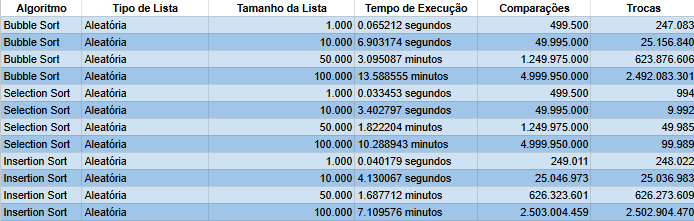
\includegraphics[width=0.9\textwidth]{listas/aleatorio4.png}
    \caption{Distribuição Aleatória Bubble Sort, Selection Sort e Insertion Sort}
    \label{fig:aleatorio4}
\end{figure}

\begin{figure}[H]
    \centering
    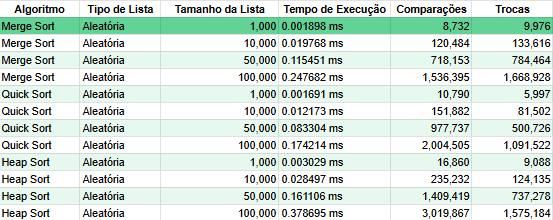
\includegraphics[width=0.9\textwidth]{listas/aleatoriom.png}
    \caption{Distribuição Aleatória Merge Sort, Quick Sort, Heap Sort}
    \label{fig:aleatoriom}
\end{figure}

\section{Listas Ordenadas}
	\textbf{Insertion Sort} é o algoritmo que apresenta o melhor desempenho nesse cenário. Como ele percorre a lista apenas verificando se os elementos estão em ordem e não realiza trocas desnecessárias, seu tempo de execução é extremamente baixo, mesmo em listas com grande número de elementos.

\textbf{Merge Sort} também apresenta desempenho muito bom em listas ordenadas. Apesar de sempre operar com complexidade $O(n \log n)$, o número de comparações e trocas permanece relativamente baixo, garantindo uma execução eficiente.

 \textbf{Quick Sort} mostra um desempenho razoável, mas inferior ao Merge Sort e ao Insertion Sort. Ele depende fortemente da escolha do pivô e, em listas ordenadas, pode realizar mais comparações e trocas do que o necessário.

\textbf{Heap Sort} mantém um desempenho estável, mas realiza muitas comparações e trocas desnecessárias, pois sempre reconstrói a heap independentemente da ordem inicial da lista, o que gera uma sobrecarga de processamento.

\textbf{Selection Sort} e \textbf{Bubble Sort} não se beneficiam do fato de a lista já estar ordenada. Embora não realizem trocas nesse caso, continuam realizando o mesmo número de comparações que fariam em uma lista desordenada, o que resulta em tempos de execução elevados e pouca eficiência.

\begin{figure}[H]
    \centering
    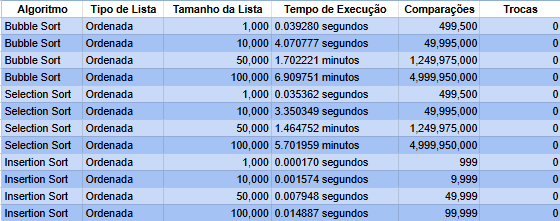
\includegraphics[width=0.9\textwidth]{listas/ordenadab.png}
    \caption{Distribuição Ordenada (Insertion e Quick)}
    \label{fig:ordenadab}
\end{figure}
\begin{figure}[H]
    \centering
    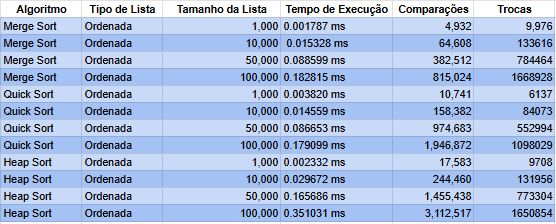
\includegraphics[width=0.9\textwidth]{listas/ordenadam.png}
    \caption{Distribuição Ordenada (Bubble e Selection)}
    \label{fig:ordenadam}
\end{figure}
\

\section{Listas Inversamente Ordenadas}
A análise dos resultados com listas inversamente ordenadas revela diferenças marcantes entre os algoritmos testados:

\begin{itemize}
    \item \textbf{Insertion Sort} sofre um impacto significativo nesse cenário, pois precisa deslocar cada elemento para a posição correta, resultando em um número muito alto de comparações e trocas. Esse é o pior caso para esse algoritmo.

    \item \textbf{Bubble Sort} também apresenta desempenho muito ruim em listas inversas, já que precisa fazer múltiplas passagens e trocas consecutivas até alcançar a ordenação correta. Ele é sensível à ordem inicial dos dados.

    \item \textbf{Selection Sort}, apesar de ter complexidade $O(n^2)$, é menos afetado pela ordem inicial, porque sempre procura o menor elemento e coloca na posição correta, independentemente da configuração inicial. Ainda assim, o desempenho geral permanece ruim para listas grandes.

    \item \textbf{Merge Sort} mantém uma performance robusta mesmo no pior caso, já que sua abordagem de dividir e conquistar não depende da ordem dos elementos. Ele garante um comportamento consistente, com baixa sensibilidade à ordem inicial.

    \item \textbf{Quick Sort} apresenta desempenho estável, mas pode degradar se o pivô não for bem escolhido. Em listas inversas, estratégias de pivô simples podem levar a mais comparações e trocas, mas o impacto ainda é moderado.

    \item \textbf{Heap Sort} também mantém boa performance e mostra-se estável nesse cenário, já que a estrutura de heap não depende da ordem inicial. No entanto, ele realiza muitas trocas e comparações internas, o que mantém sua execução um pouco mais pesada do que a do Merge Sort.

\end{itemize}

\begin{figure}[H]
    \centering
    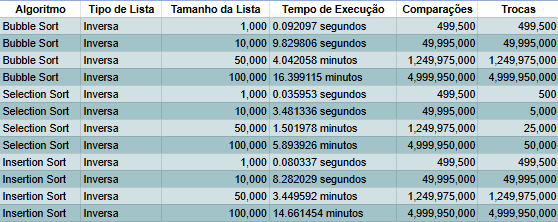
\includegraphics[width=0.9\textwidth]{listas/inversab.png}
    \caption{Distribuição Inversa (Insertion e Quick)}
    \label{fig:inversab}
\end{figure}
\begin{figure}[H]
    \centering
    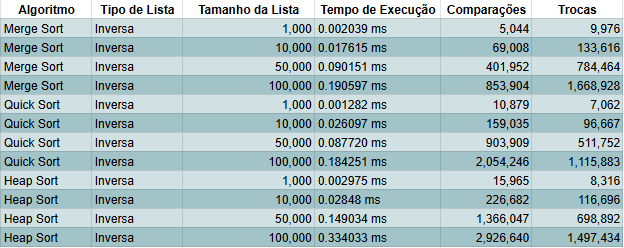
\includegraphics[width=0.9\textwidth]{listas/inversam.png}
    \caption{Distribuição Inversa (Bubble e Selection}
    \label{fig:inversam}
\end{figure}



% Discussão
\chapter{Discussão}

\begin{enumerate}
    \item \textbf{Heap Sort e Merge Sort}
    \begin{itemize}
        \item Heap Sort e Merge Sort apresentam desempenho consistente devido à sua complexidade $O(n \log n)$, destacando-se em listas de grande porte. Esses algoritmos mantêm boa eficiência independentemente da distribuição inicial dos dados, sendo apropriados para situações em que é necessário lidar com grandes volumes de informação.
    \end{itemize}

    \item \textbf{Quick Sort}
    \begin{itemize}
        \item Quick Sort também é muito eficiente na prática, especialmente em listas aleatórias. No entanto, seu desempenho pode se degradar em listas já ordenadas ou quase ordenadas, devido à escolha do pivô, que influencia diretamente o número de comparações e a profundidade da recursão.
    \end{itemize}

   
\end{enumerate}

\section{Facilidade de Implementação e Estabilidade}

\subsection{Facilidade de Implementação}
\begin{itemize}
    \item Bubble Sort, Selection Sort e Insertion Sort são fáceis de implementar, devido à simplicidade de sua lógica. Contudo, essa facilidade vem à custa de baixo desempenho.
    \item Heap Sort e Quick Sort requerem uma implementação mais sofisticada, envolvendo operações como particionamento (Quick Sort) e manutenção da estrutura de heap (Heap Sort).
    \item Merge Sort, apesar de simples de implementar recursivamente, exige cuidados adicionais no gerenciamento do espaço de memória extra.
\end{itemize}

\subsection{Estabilidade}
\begin{itemize}
    \item Merge Sort é estável, preservando a ordem relativa de elementos iguais, característica importante em aplicações específicas.
    \item Quick Sort e Heap Sort não são estáveis, podendo alterar a ordem dos elementos iguais durante o processo de ordenação.
    \item Bubble Sort e Insertion Sort são estáveis, o que os torna úteis em cenários onde a estabilidade é fundamental, apesar de sua baixa eficiência em listas extensas.
\end{itemize}


\section{Discussão sobre pontos a melhorar e alguns aspectos dos algoritmos}

Os resultados obtidos nos experimentos permitem observar de forma clara o comportamento de cada algoritmo em diferentes cenários de entrada:

\begin{enumerate}
    \item \textbf{Bubble Sort} e \textbf{Selection Sort} demonstram ser altamente ineficientes para listas de grande porte, independentemente da ordenação inicial dos dados. Ambos mantêm complexidade \(O(n^2)\) em número de comparações mesmo em listas já ordenadas, o que evidencia a limitação estrutural desses algoritmos. No caso do Bubble Sort, embora o número de trocas caia a zero em listas ordenadas, o número de comparações permanece elevado, o que compromete a eficiência geral. Esses resultados empíricos estão em linha com a teoria, que sugere que esses algoritmos são ineficientes em listas grandes, especialmente em cenários desfavoráveis como listas inversamente ordenadas. Em contextos reais, algoritmos mais eficientes como Merge Sort, Quick Sort ou algoritmos híbridos (como o Timsort) são preferidos.
    
    \item \textbf{Insertion Sort}, por outro lado, destaca-se positivamente em listas ordenadas ou quase ordenadas, apresentando complexidade próxima de \(O(n)\). Isso se deve ao fato de que, nesses casos, o algoritmo praticamente não realiza trocas, e as comparações são minimizadas, o que explica os tempos extremamente baixos registrados nesses cenários. Esse comportamento o torna particularmente vantajoso em aplicações onde os dados tendem a estar quase organizados. A teoria confirma esse comportamento, com o algoritmo apresentando um desempenho significativamente melhor em listas parcialmente ordenadas. No entanto, sua performance diminui em listas aleatórias ou inversamente ordenadas, o que é esperado dado seu pior caso de \(O(n^2)\).
    
    \item A ordenação inicial dos dados exerce forte influência no desempenho dos algoritmos. Listas inversamente ordenadas representam o pior caso para todos os métodos testados, especialmente para o Insertion Sort e o Bubble Sort, que precisam realizar um número máximo de comparações e trocas para ordenar os elementos. Em contraste, listas já ordenadas representam o melhor caso para o Insertion Sort, onde seu tempo de execução se torna praticamente desprezível mesmo em listas com 100.000 elementos. Isso é confirmado pela teoria, que explica como a quantidade de trocas e comparações realizadas depende diretamente da ordenação inicial dos dados.
    
    \item \textbf{Limitações e Recomendações}:
    \begin{itemize}
        \item Embora os algoritmos Bubble Sort, Selection Sort e Insertion Sort sejam úteis do ponto de vista didático, sua aplicação em larga escala não é recomendada devido ao seu alto custo computacional em cenários desfavoráveis. A comparação entre os resultados empíricos e teóricos mostra que, embora simples de implementar, esses algoritmos se tornam ineficazes à medida que o tamanho da lista aumenta.
        
        \item Em cenários do mundo real, algoritmos como \textbf{Merge Sort} e \textbf{Quick Sort} são preferidos por sua melhor eficiência. Esses algoritmos possuem complexidade \(O(n \log n)\), o que os torna muito mais adequados para aplicações de larga escala. A inclusão de outros algoritmos mais eficientes, como o \textbf{Timsort} (usado em Python), pode ser uma boa sugestão para melhorar o desempenho em listas grandes.
    \end{itemize}
    
    \item \textbf{Sugestões para Estudos Futuros}: 
    \begin{itemize}
        
        \item Analisar o consumo de memória de algoritmos como o \textbf{Quick Sort} e o \textbf{Merge Sort} para entender melhor o impacto de seu uso de memória em comparação com algoritmos mais simples.
        
        \item Estudar alternativas como \textbf{Radix Sort}, que também têm complexidade \(O(n \log n)\) e podem ser mais eficientes em certos contextos de dados.
    \end{itemize}
\end{enumerate}
\section*{Bubble Sort}

\textbf{Como funciona:}
\begin{itemize}
    \item Laço externo: passa $n$ vezes pela lista.
    \item Laço interno: compara elementos adjacentes até o final da lista (diminuindo a cada passo).
\end{itemize}

\[
\text{for } i \text{ in range}(n): 
\quad \text{for } j \text{ in range}(0, n - i - 1):
\quad \text{if } arr[j] > arr[j+1]:
\quad \text{trocar}
\]

\textbf{Quantas comparações?}

\begin{itemize}
    \item No 1º passo, compara $n - 1$ pares: $arr[0]$ com $arr[1]$, até $arr[n-2]$ com $arr[n-1]$.
    \item No 2º passo, $n - 2$ comparações (último já está no lugar).
    \item \dots
    \item No último passo, 1 comparação.
\end{itemize}

A soma das comparações é:

\[
(n-1) + (n-2) + \dots + 1 = \frac{n(n-1)}{2} \quad \Rightarrow \quad O(n^2)
\]

\textbf{Trocas:}
No pior caso (lista invertida), cada comparação resulta em uma troca, logo também temos $O(n^2)$.

\section*{Selection Sort}

\textbf{Como funciona:}
\begin{itemize}
    \item Para cada posição $i$, você procura o menor elemento no resto da lista.
    \item Quando encontra, faz uma única troca no final da rodada.
\end{itemize}

\[
\text{for } i \text{ in range}(n):
\quad \text{min\_index} = i
\quad \text{for } j \text{ in range}(i+1, n):
\quad \text{if } arr[j] < arr[min\_index]:
\quad \text{min\_index} = j
\quad \text{trocar } arr[i] \text{ com } arr[min\_index]
\]

\textbf{Quantas comparações?}

\begin{itemize}
    \item 1ª rodada: compara $n - 1$ elementos.
    \item 2ª rodada: $n - 2$ comparações.
    \item \dots
    \item Última: 1 comparação.
\end{itemize}

A soma das comparações é:

\[
(n-1) + (n-2) + \dots + 1 = \frac{n(n-1)}{2} \quad \Rightarrow \quad O(n^2)
\]

\textbf{Trocas:}
Uma única troca por rodada (mesmo se não precisar).

\[
\text{Máximo: } n - 1 \text{ trocas} \quad \Rightarrow \quad O(n)
\]

\section*{Insertion Sort}

\textbf{Como funciona:}
\begin{itemize}
    \item Vai inserindo cada elemento no lugar certo da parte já ordenada.
    \item Compara com os elementos anteriores até achar onde encaixar.
\end{itemize}

\[
\text{for } i \text{ in range}(1, n):
\quad \text{chave} = arr[i]
\quad j = i - 1
\quad \text{while } j \geq 0 \text{ and } arr[j] > \text{chave}:
\quad arr[j+1] = arr[j]
\quad j -= 1
\quad arr[j+1] = \text{chave}
\]

\textbf{Quantas comparações?}

\begin{itemize}
    \item No melhor caso (lista já ordenada), $arr[j] > \text{chave}$ nunca é verdade, logo só uma comparação por $i$.
    \item Total: $n - 1$ comparações, logo $O(n)$.
    \item No pior caso (lista invertida), cada chave é menor que todos os anteriores.
    \item 1ª inserção: 1 comparação.
    \item 2ª: 2 comparações.
    \item \dots
    \item Última: $n - 1$ comparações.
\end{itemize}

A soma das comparações é:

\[
1 + 2 + \dots + (n - 1) = \frac{n(n - 1)}{2} \quad \Rightarrow \quad O(n^2)
\]


\chapter{Conclusão}

A análise experimental realizada com os algoritmos de ordenação Bubble Sort, Selection Sort, Insertion Sort, Merge Sort, Quick Sort e Heap Sort revelou diferenças significativas de desempenho em termos de tempo de execução, número de comparações e número de trocas, especialmente à medida que o tamanho das listas aumentava.

Os algoritmos Bubble Sort, Selection Sort e Insertion Sort, todos de complexidade $O(n^2)$, apresentaram tempos de execução extremamente elevados em listas com 50.000 ou 100.000 elementos, chegando a consumir vários minutos. O Bubble Sort destacou-se negativamente pelo altíssimo número de trocas, mesmo em listas ordenadas e inversamente ordenadas, evidenciando sua baixa eficiência prática. O Selection Sort, embora também apresente alto custo em comparações, realizou pouquíssimas trocas, o que o torna previsível, mas não necessariamente eficiente. O Insertion Sort, por sua vez, apresentou bom desempenho em listas ordenadas, mas sofreu grande degradação com o aumento do tamanho e da desordem dos dados.

Os algoritmos de complexidade $O(n \log n)$ — Merge Sort, Quick Sort e Heap Sort — mostraram-se muito mais adequados para lidar com listas grandes. O Merge Sort foi consistente e estável, com baixíssimo tempo de execução mesmo em listas grandes, e sem realizar trocas no sentido clássico, o que é característico de seu funcionamento baseado em cópias e fusões. O Quick Sort apresentou excelente desempenho em quase todos os cenários, mas é importante destacar que seu desempenho depende fortemente da escolha do pivô, o que pode ser um ponto fraco em casos desfavoráveis. O Heap Sort mostrou-se robusto e competitivo, combinando um número controlado de comparações e trocas, independentemente da ordem inicial da lista.

Em termos de comparações, os algoritmos quadráticos foram, como esperado, muito menos eficientes do que os algoritmos $O(n \log n)$, chegando a ultrapassar bilhões de comparações nas listas maiores. Já em termos de trocas, os resultados variaram: enquanto Bubble Sort foi extremamente ineficiente, o Merge Sort apresentou virtualmente zero trocas, e Heap Sort manteve um equilíbrio notável.

De modo geral, os resultados confirmam que algoritmos $O(n \log n)$ são preferíveis para aplicações práticas envolvendo grandes volumes de dados, enquanto os algoritmos quadráticos devem ser utilizados apenas para fins didáticos ou em contextos específicos, como listas pequenas ou parcialmente ordenadas. Esta análise reforça a importância de compreender as características internas de cada algoritmo, permitindo uma escolha informada de acordo com as necessidades e limitações do problema.





% Referências
\chapter*{Referências}
\addcontentsline{toc}{chapter}{Referências}


    Cormen, T. H., Leiserson, C. E., Rivest, R. L., \& Stein, C. (2009). 			    {Introduction to Algorithms}. MIT Press.
    Sedgewick, R., \& Wayne, K. (2011). \textit{Algorithms}. Addison-Wesley.


\end{document}



